\chapter{\xlabel{pol2_dr}POL-2 Data Reduction - The Theory}
\label{sec:dr}
\section{\xlabel{dataflow}The Data Flow}

POL-2 data reduction is a complex and involved process
for which a borad overview is presented first before
the specific details are discussed.



\begin{figure}[t!]
\begin{center}
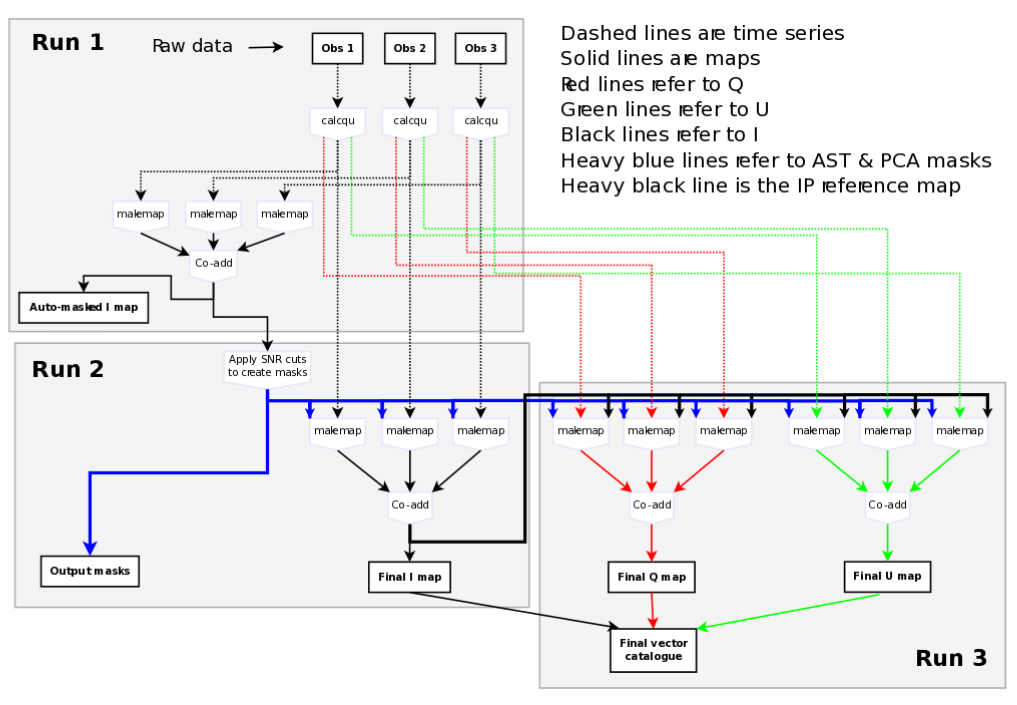
\includegraphics[width=0.95\linewidth]{pol2-dr-flow.png}
\label{fig:pol2drflow}
\caption [POL-2 Data Flow]{
  \small The data flow of the POL-2 data reduction method is
  presented. In this example three POL-2 observations are
  reduced and combined in various stages and combinations to
  produce I, Q and U maps.
}
\end{center}
\end{figure}

\subsection*{Step 1}

\subsection*{Step 2}

\subsection*{Step 3}



\section{\xlabel{makemap}Makemap}

The POL-2 data reduction builds upon the SCUBA-2 data reduction

\cite{smurf}

\section{\xlabel{pca}PCA}


\section{\xlabel{masking}Masking}


\section{\xlabel{addingdata}Adding new observations}



\section{\xlabel{tailoredDR}Tailoring your reduction}


